\documentclass[tikz]{standalone}

\usepackage{tikz,tkz-euclide}
\usepackage{pgfplots}
\usepackage{pgfplotstable}
\pgfplotsset{compat=newest}
\usepgfplotslibrary{fillbetween}

\begin{document}
	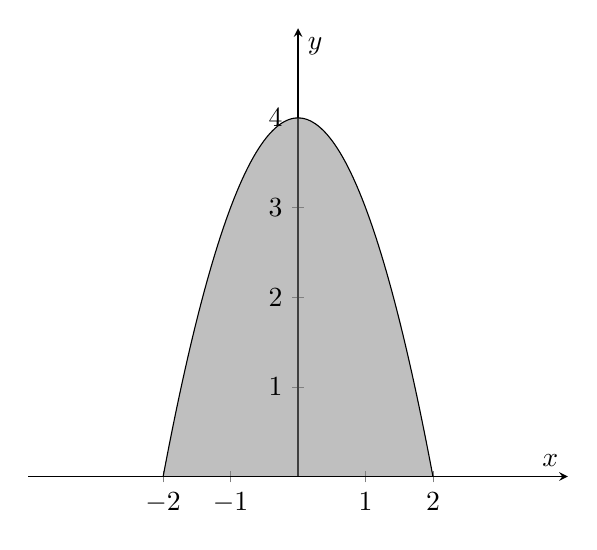
\begin{tikzpicture}
		\begin{axis}[
			xmin=-4,xmax=4,ymin=0,ymax=5,
			axis line style={->},
			%ticks=none,
			xlabel=$x$,ylabel=$y$,
			%xlabel style={at=right},
			%ylabel style={at=above},
			axis x line=middle,
			axis y line=middle,
			xtick={-2,-1,0,1,2},ytick={0,1,2,3,4}
			]
			\addplot [domain=-2:2, samples=100, name path=f] {-x*x+4};
			\addplot [name path=xaxis] (-2,0) -- (2,0);
			\addplot [gray, opacity=0.5] fill between [of=f and xaxis, soft clip={domain=-2:2}];
		\end{axis}
	\end{tikzpicture}
\end{document}
